\documentclass{article}
\usepackage{t1enc}
%\usepackage[latin2]{inputenc}
\usepackage[utf8]{inputenc}
\usepackage[magyar]{babel}
\usepackage{amsmath, amssymb, amsfonts}
%\usepackage[colorlinks=true]{hyperref}
\frenchspacing
\usepackage{graphicx}
\usepackage{pdfpages}
\usepackage{float}


\title{Leíró és matematikai statisztika $2018$/$2019$ II. félév beadandó feladat}
\author{Bedő Botond}
\date{\today}
\pagestyle{headings}


\begin{document}
\maketitle
\newpage	

\section{A vizsgált adatok rövid bemutatása}
\subsection{Az adathalmaz bemutatása}
Az adathalmaz Amerikában $2012$ és $2014$ között bekövetkezett fegyverek által okozott halálokról tartalmaz információt. Az adathalmaz összesen 100798 adatot tartalmaz, amiket $11$ változó alapján jegyeztek fel. Azok az adattagok, melyek nem ismertek, NA-val vannak helyettesítve.

\subsection{Változók bemutatása}

\begin{itemize}
	\item ID: adatok sorszáma
	\item year: a haláleset bekövetkeztének éve, $2012-2014$ között
	\item month: a haláleset melyik hónapban következett be, számokkal jelölve
	\item intent: a haláleset oka, lehet Accidental (baleset); Homicide (gyilkosság); Suicide (öngyilkosság); Undeterminded (nemmeghatározott)
	\item police: rendőr részt vett-e a lövöldözésben, logikai változó, lehet $1$ (igaz); $0$ (hamis) 
	\item sex: az áldozat neme, M (férfi); F (nő)
	\item age: az áldozat kora
	\item race: az áldozat rassza, lehet Asian/Pacific Islander; White; Native American/Native Alaskan; Black; Hispanic
	\item hispanic: számmal jelölt kód, ami az áldozat hispan származására utal
	\item place: a haláleset helyszíne: Farm (farm); Home (áldozat otthona); Industrial/construction (ipari/építkezési terület); Other specified (egyéb meghatározott); Other unspecified (egyéb nemmeghatározott); Residential institution (lakossági intézmény); School/institution (iskola); Sports (sportolási helyszín); Street (utca); Trade/service area (kereskedelmi/szolgáltatási terület)
	\item education: az áldozat műveltségi szintje, számbeli adat, lehet $1$ (Érettségi nélküli); $2$ (Érettségivel rendelkező); $3$ (Egyetemi képzésben részesült); $4$ (Egyetemi végzettséggel rendelkezik); $5$ (nem ismert)
\end{itemize}

\subsection{Az adathalmaz tisztítása, és szűrése}

Azokat az adatokat, amelyek tartalmaznak ismeretlen ($NA$) adattagokat, kitöröltem. Azokat az adatokat, amelyeknél az intent változó értéke Undetermined, vagy az education értéke $5$, kitöröltem. Ezek után $97218$ darab adatom maradt, vagyis az eredeti $100798$-nek nagyjából a $3.55\%$-át töröltem csak ki, ami közel százezres nagyságrendű adathalmaznál jelentéktelen mennyiség. \par
A változók közül eltávolítottam a következőket:
\begin{itemize}
	\item ID, mert az R automatikusan elvégzi a sorszámozást
	\item police, mert eredetileg is csak $19$ alkalommal veszi fel az 1-es értéket, (amikor jelen volt rendőr is) ami közel százezer adathalmaznál jelentéktelen mennyiség, nem lehet belőle következtetni
	\item hispanic, mert nem egyértelmű a jelentése
\end{itemize}
\par
Ezek után összesen $8$ változó maradt.

\section{Az adatsor áttekintése egyszerű ábrákkal}
\subsection{Fegyver általi halálok eloszlása évenkénti, majd hónaponkénti bontásban}

\begin{figure}[h]
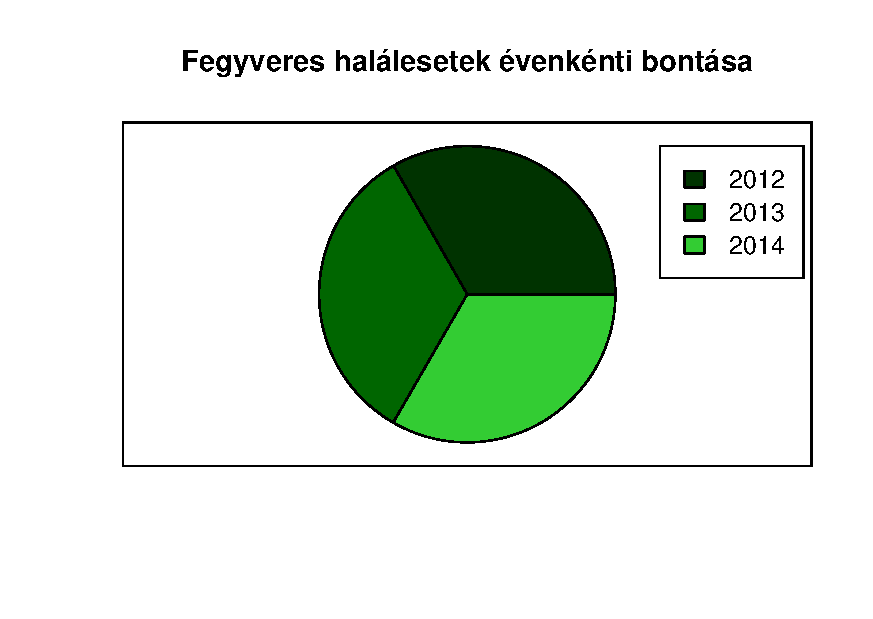
\includegraphics[width=65mm]{plot1.pdf}
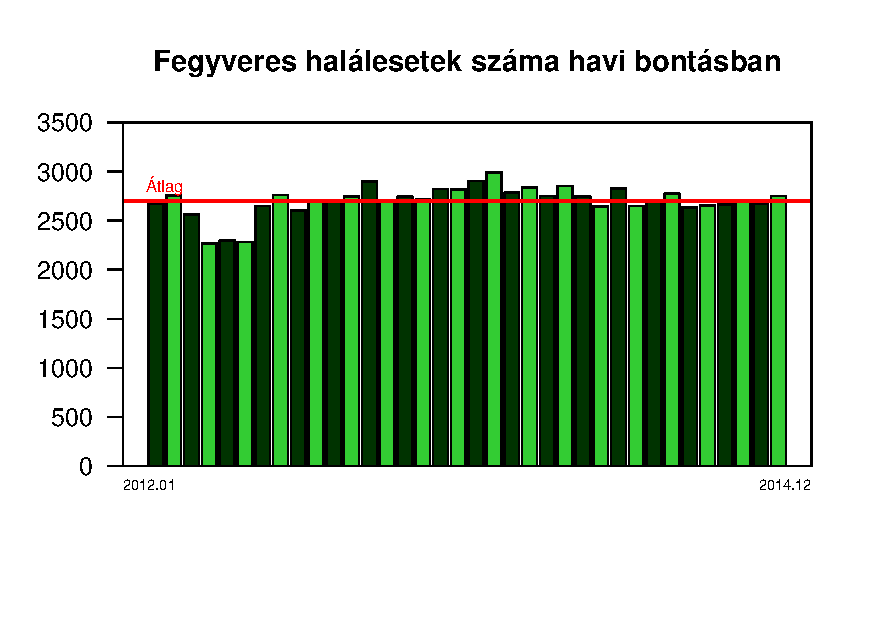
\includegraphics[width=65mm]{plot2.pdf}
\end{figure}

A halálesetek arányosan oszlanak el az időben, mind az évenkénti, mind a hónaponkénti bontást vizsgálva, ritkák az átlagtól való eltérések, és nem is szignifikánsak.

\subsection{A nemek aránya az áldozatok közt}

\begin{minipage}{0.5\textwidth}
\begin{figure}[H]
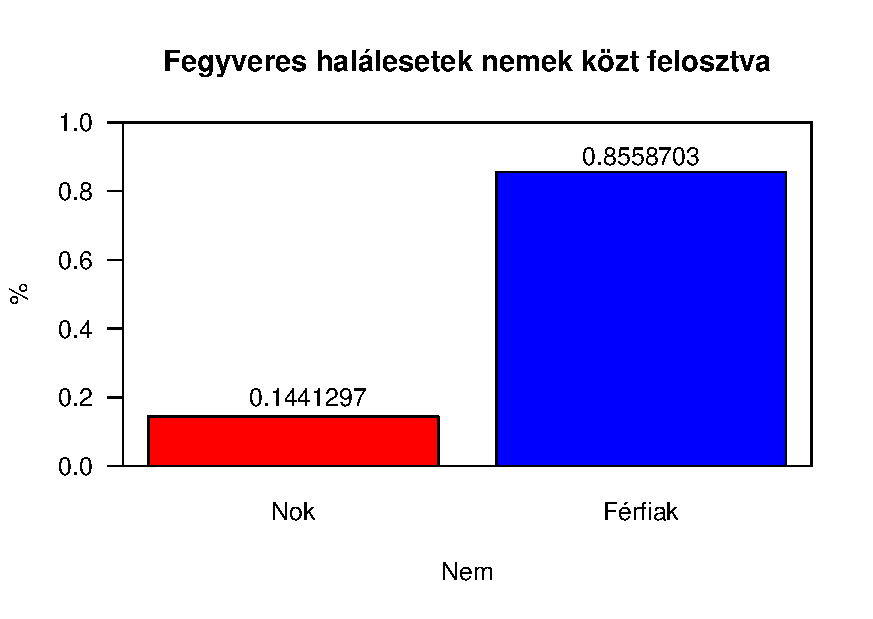
\includegraphics[width=65mm]{plot3.pdf}
\end{figure}
\end{minipage} \hfill
\begin{minipage}{0.45\textwidth}
Az adatok alapján férfiak sokkal nagyobb számban halnak meg fegyver által mint nők, ez az adatbázis $14012$ nőt és  $83206$ férfit tartalmaz.
\end{minipage}


\subsection{A fegyverhasználat célja szerinti arányok}

\begin{minipage}{0.45\textwidth}
Az öngyilkosság közel kétszer olyan gyakran fordul elő az adatok közt, mint a gyilkosság, a baleseti gyilkosságok sokkal kevesebbszer fordulnak elő a másik két kimenetelnél, körülbelül az adatok $1.5\%$-át fedi le, ami nem egy elhanyagolható létszám, ez körülbelül $1458$ halálos áldozat.
\end{minipage}
\begin{minipage}{0.5\textwidth}
\begin{figure}[H]
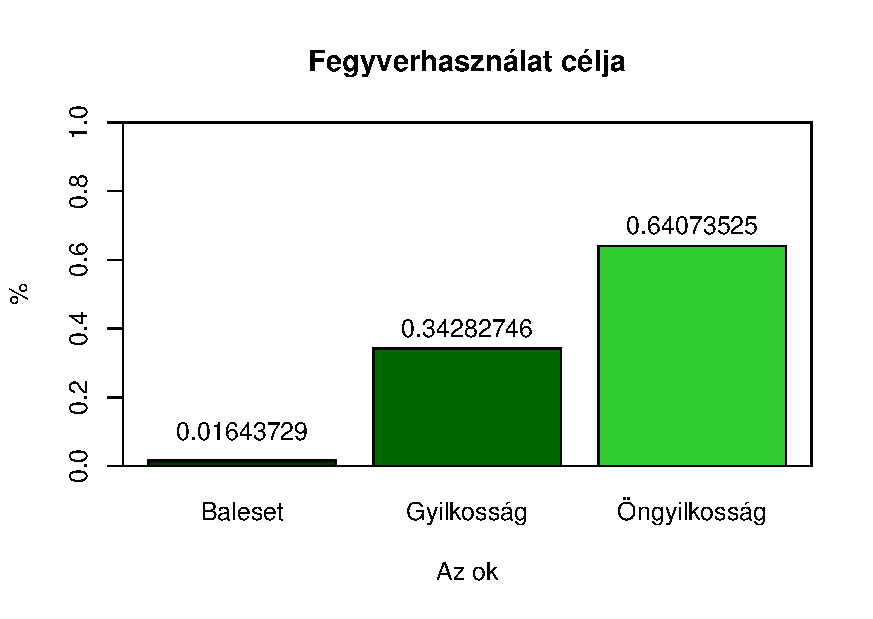
\includegraphics[width=65mm]{plot4.pdf}
\end{figure}
\end{minipage} \hfill

\subsection{Műveltségi szint alapján történő bontás}

\begin{minipage}{0.5\textwidth}
\begin{figure}[H]
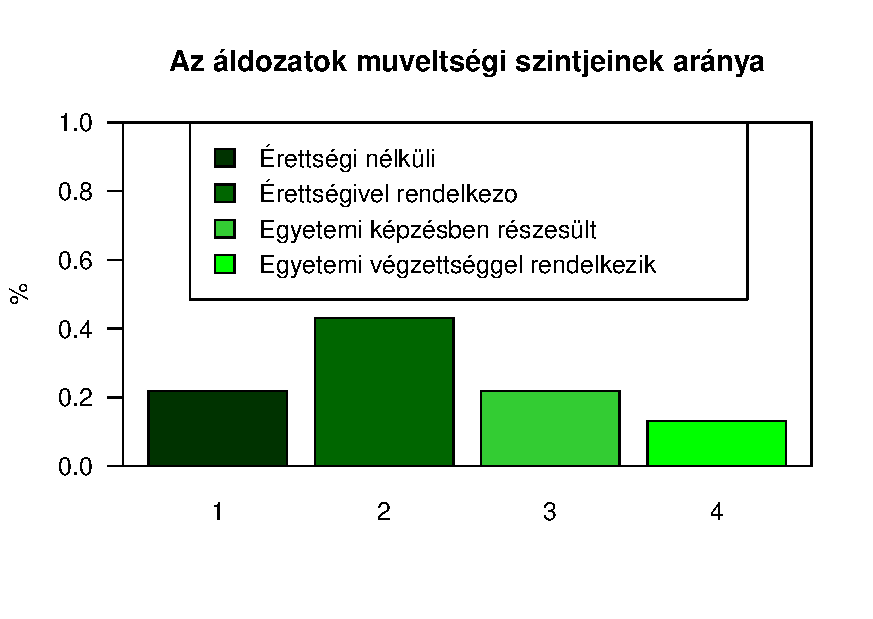
\includegraphics[width=65mm]{plot5.pdf}
\end{figure}
\end{minipage} \hfill
\begin{minipage}{0.45\textwidth}
Az adatok azt mutatják, hogy kevesebb az iskolázottabb áldozat, azt viszont ezek alapján nem lehet eldönteni, hogy azért, mert a tanultabb emberek általában biztonságosabb környezetben helyezkednek el, vagy azért, mert arányaiban is kevesebb ember rendelkezik egyetemi képzéssel, mint amennyi nem.
\end{minipage}

\subsection{Rassz alapján történő vizsgálat}

\begin{minipage}{0.45\textwidth}
Jelentősen kiemelkedik a fehér áldozatokról szóló adat, továbbá a fehérekről, a feketékről és hispanokról szóló adatok lefedik a halálesetek $98\%$-át, emiatt a többi rasszról szóló adat túl kevés, hogy lényegi következtetéseket lehessen belőle levonni.
\end{minipage}
\begin{minipage}{0.5\textwidth}
\begin{figure}[H]
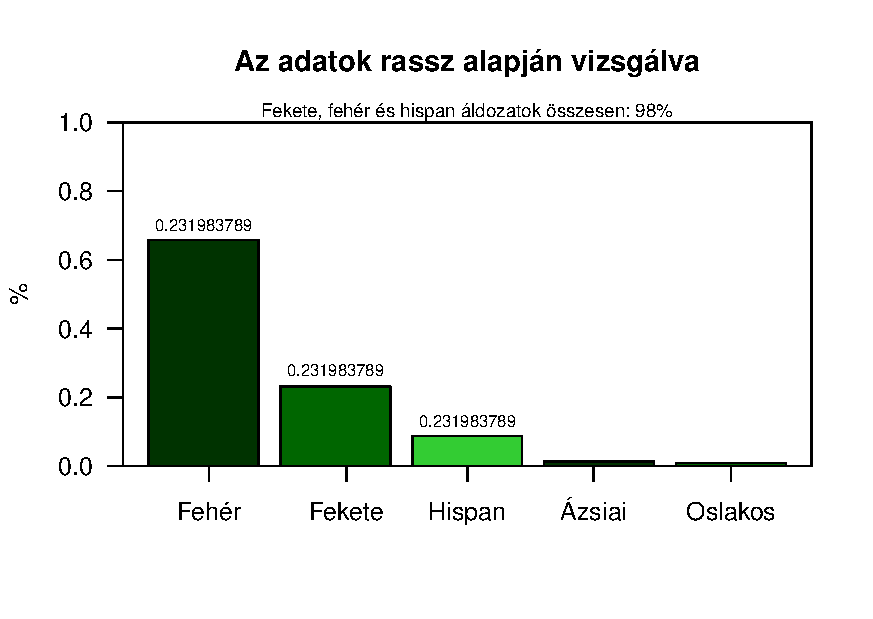
\includegraphics[width=65mm]{plot6.pdf}
\end{figure}
\end{minipage} \hfill

\subsection{Helyszínenkénti bontás}

\begin{minipage}{0.5\textwidth}
\begin{figure}[H]
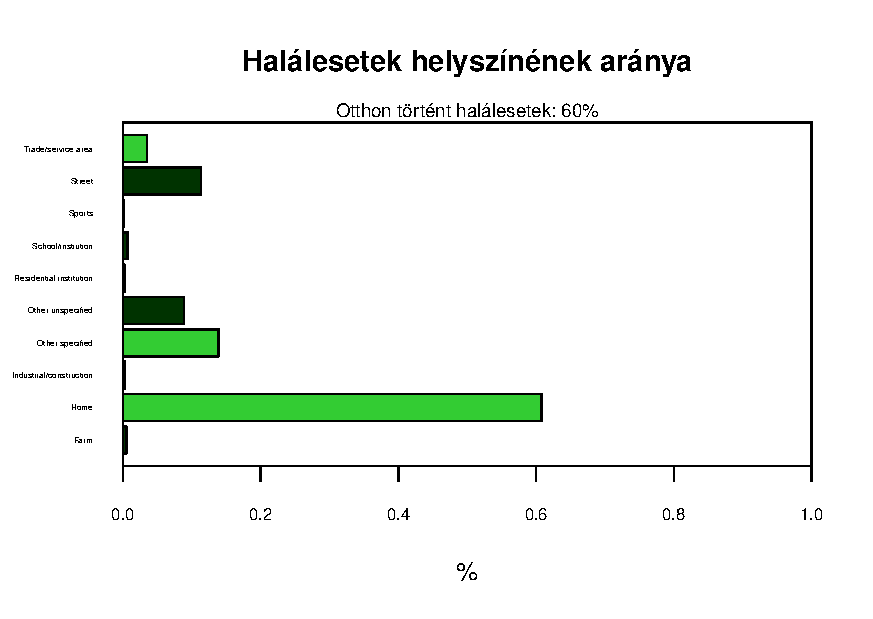
\includegraphics[width=65mm]{plot7.pdf}
\end{figure}
\end{minipage} \hfill
\begin{minipage}{0.45\textwidth}
Otthoni halálesetek fordulnak elő kiemelkedő gyakorisággal, az esetek $60\%$-ában az összesen $10$ lehetőség közül. A legtöbb helyszín alapján nehéz következtetéseket levonni a hozzájuk tartozó viszonylag kevés adat miatt.
\end{minipage}

\section{Adatsorok egyedi elemzése}

\subsection{Fegyveres halálesetek kor alapján ábrázolva, majd szándék alapján szétválasztva}

\begin{figure}[h]
\centering
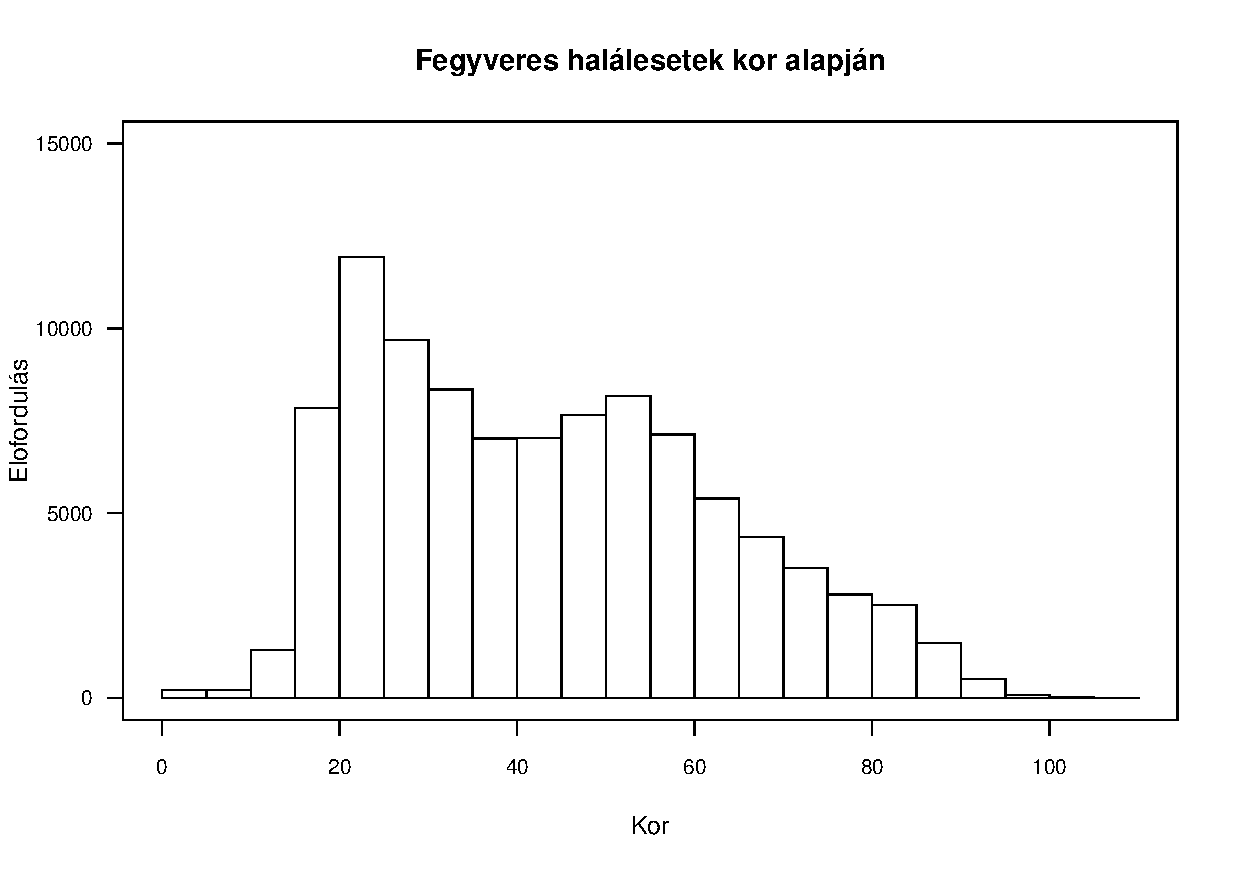
\includegraphics[width=100mm]{plot8.pdf}
\end{figure}

A $15.$ életév betöltése után a fegyver általi halálok száma jelentősen megugrik, és az egész histogramot tekintve egy tüske fedezhető fel az adatok ezen részén. A $20$ - $25$ éves korosztály tartalmazza a legtöbb adatot, majd a tüske után, a $35$ - $45$ év közöttieknél visszaesés figyelhető meg. A visszaesést egy apró emelkedés követi, ami után, az $55.$ évüket betöltöttek után közel egyenletesen csökken a halálesetek száma, egészen a histogram végéig. \par
Érdemes lehet hasonló histogramokat vizsgálni, a gyilkosság célja alapján különválasztva az adatokat.

\begin{minipage}{0.45\textwidth}
Az önygyilkosságokat tartalmazó adatok eloszlása normálisabbnak néz ki, mint az egész adathalmaz, nincsenek kiugró adatcsoportok, $30$ - $40$ év közti apró süllyedést leszámítva az adatok száma nagyjából egyenletesen nő az $50$ év körüli korosztályig, ahonnan nagyjából egyenletesen csökken a végéig.
\end{minipage}
\begin{minipage}{0.5\textwidth}
\begin{figure}[H]
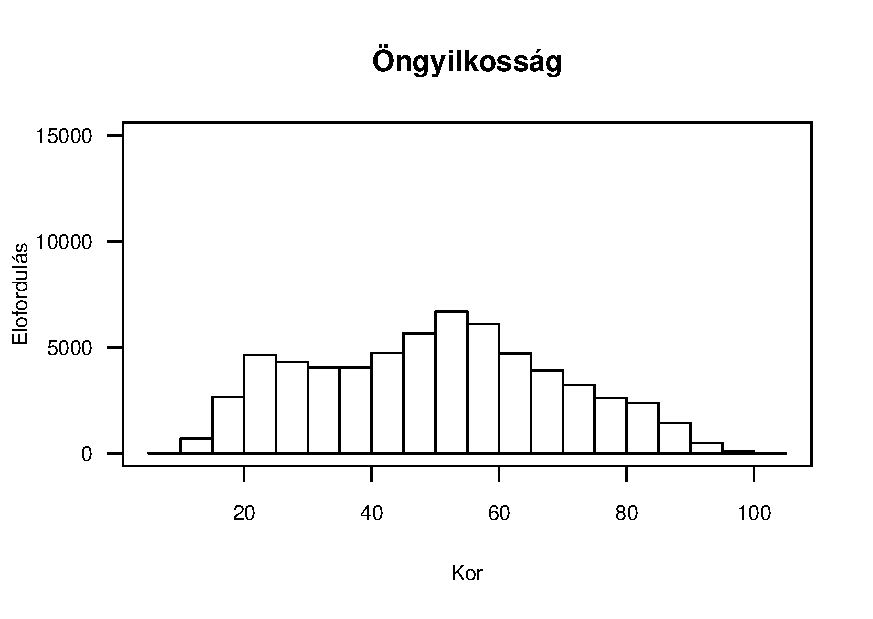
\includegraphics[width=65mm]{plot9.pdf}
\end{figure}
\end{minipage} \hfill


\begin{minipage}{0.5\textwidth}
\begin{figure}[H]
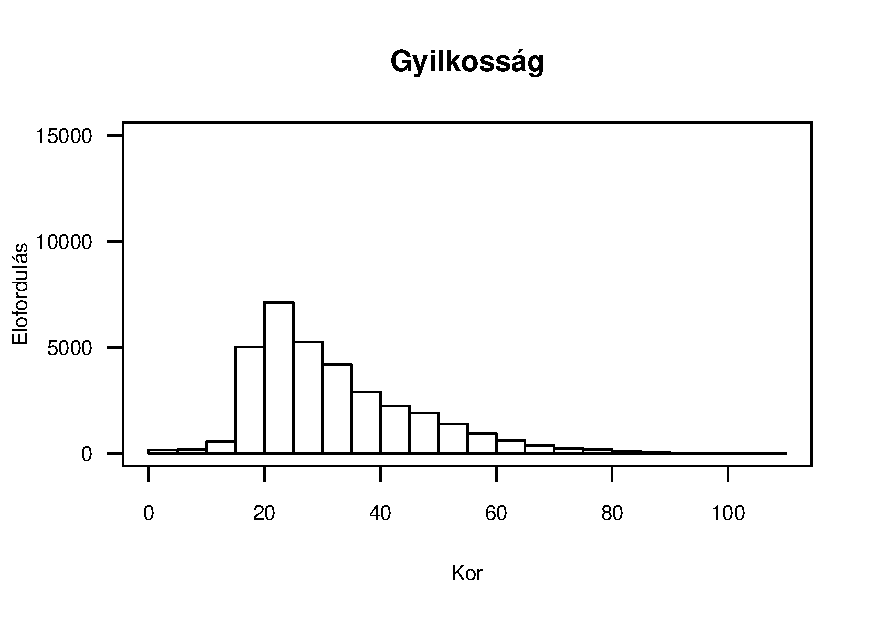
\includegraphics[width=65mm]{plot10.pdf}
\end{figure}
\end{minipage} \hfill
\begin{minipage}{0.45\textwidth}
A gyilkosságok a $15$ év alattiakat kevésbé érinti, utáni viszont jelentős ugrás található, majd az összesített adatokhoz hasonló tüske, amiből arra lehet következtetni, hogy a huszonéves korosztálynál lévő nagy halálmennyiség a gyilkosságok miatt van jelen. A tüske után, ahogy nő az életkorok csoportja, egyre kevesebb gyilkosság történik, a lineáris esetnél gyorsabban fogyatkozva, egészen az adatok végéig.
\end{minipage}

Végül, pontosabb adatok leolvasása érdekében, készítsünk egy boxplot ábrát is, ugyenezekre az adatokra, ezúttal csak az összesített esetben.

\begin{figure}[h]
\centering
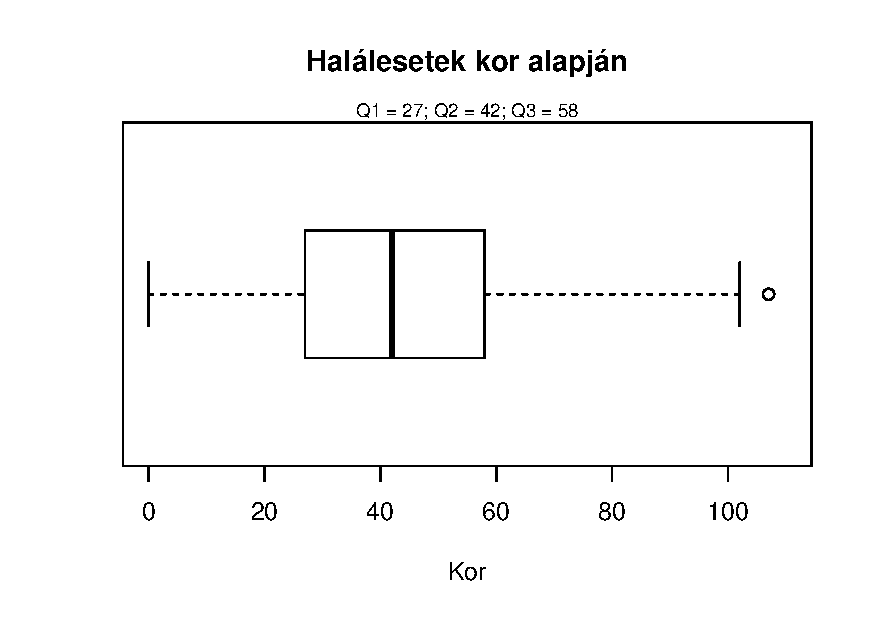
\includegraphics[width=100mm]{plot11.pdf}
\end{figure}


\subsection{Boxplot nemek alapján tördelve, műveltség alapján ábrázolva, a kor tekintetében}

\begin{figure}[h]
\centering
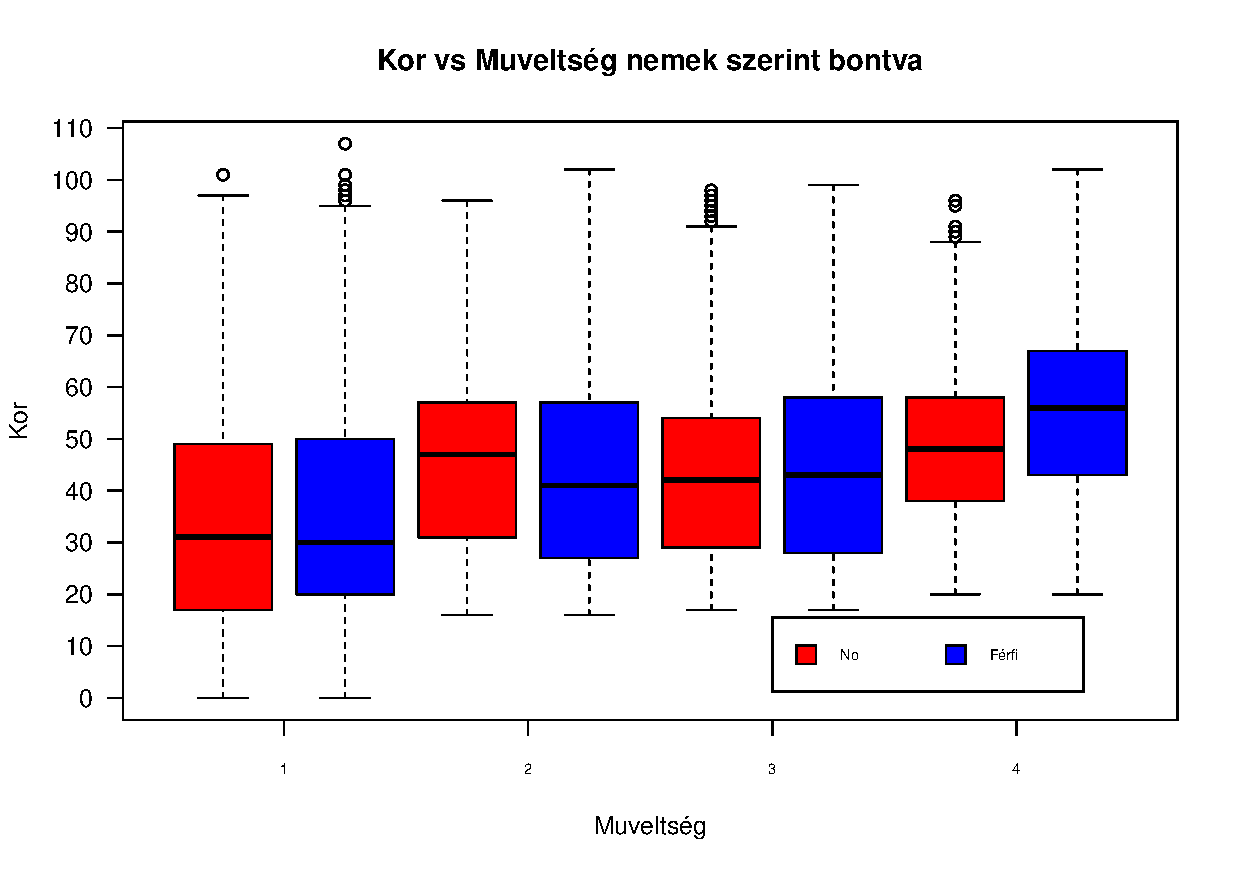
\includegraphics[width=130mm]{plot12.pdf}
\end{figure}
Az ábráról leolvasható, hogy a kevésbé iskolázottak alacsonyabb életkort élnek meg átlagosan, ami egy elvárható eredmény, ugyanis akik nagyon fiatalon halnak meg, azoknak nincs lehetőségük továbbtanulásra. Ezt jelzi az alacsonyabb átlagon túl az első kategória látványosan kisebb első kvartilise, és minimuma is. Azok közt, akik legalább részt vettek felsőoktatásban ($3.$ és $4.$ kategóriák) a férfiak életkora magasabb volt halálukkor,mint a nőké. Ezt mutatják a nőknél megjelenő kiugró értékek, az alacsonyabb maximumok, és a $4.$ kategóriánál lévő, látványos átlagéletkor különbség is.

\section{Normalitásvizsgálat}

A normalitásvizsgálatot csak Q-Q plotok alapján, és a sűrűségfüggvény alapján fogom végezni, ugyanis a Shapiro-Wilk próba ilyen nagy adathalmaz esetén már nem használható, véletlenszerű elemek kiválasztása esetén pedig erősen váltakozó eredményt ad, ugyanis az ideális adatszám, amire szüksége lenne, az adatbázisom $0.1\%$-a.

\subsection{Kor az összes adat alapján}

A kor változó a Q-Q plot alapján vastag szélű, szimmetrikus eloszlású, a normális eloszlásnál jobban leírhatja egy alacsony szabadságfokú t-eloszlás, ugyanakkor $-3$ és $-2$ között az ábra alakot vált, ami inkább egy pozitív ferdeségű szimmetrikus eloszlásra utalhat, például f-eloszlásra. A histogramon ez jól nyomon követhető az adatok terebélyességén és a huszonéveseknél lévő tüske alapján. Mivel az adathalmaz távol áll egy normális eloszlástól, érdemes bizonyos változók alapján lebontva, több részletben is megvizsgálni, hogy a hipotézisvizsgálatok pontosabb eredményeket adhassanak.

\begin{figure}[h]
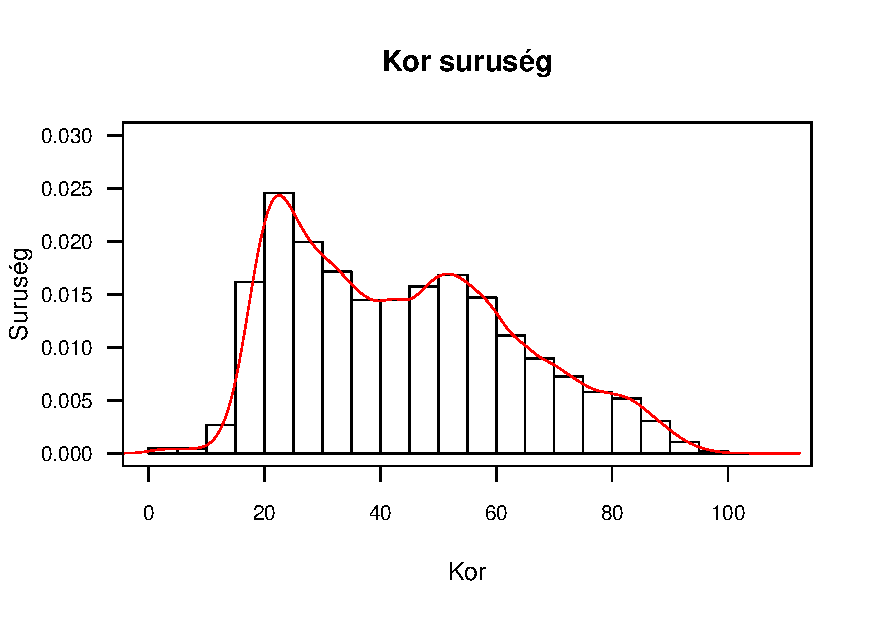
\includegraphics[width=65mm]{plot13.pdf}
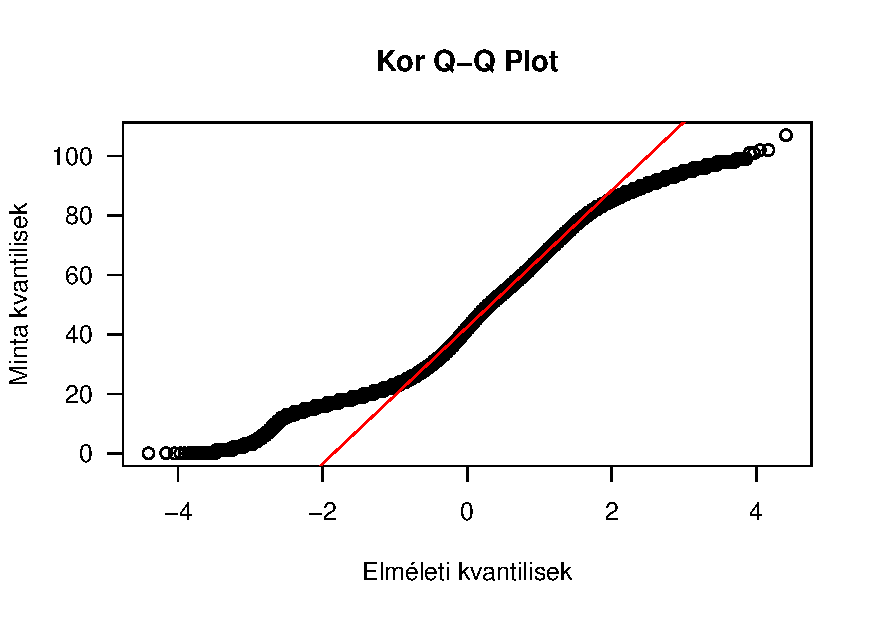
\includegraphics[width=65mm]{plot14.pdf}
\end{figure}

\subsubsection{Fehér férfiak gyilkosságban haltak meg}

Az eloszlás jobban közelíti a normális eloszlást, mint az általános eset, ám enyhán pozitív ferdeségű.

\begin{figure}[!htb]
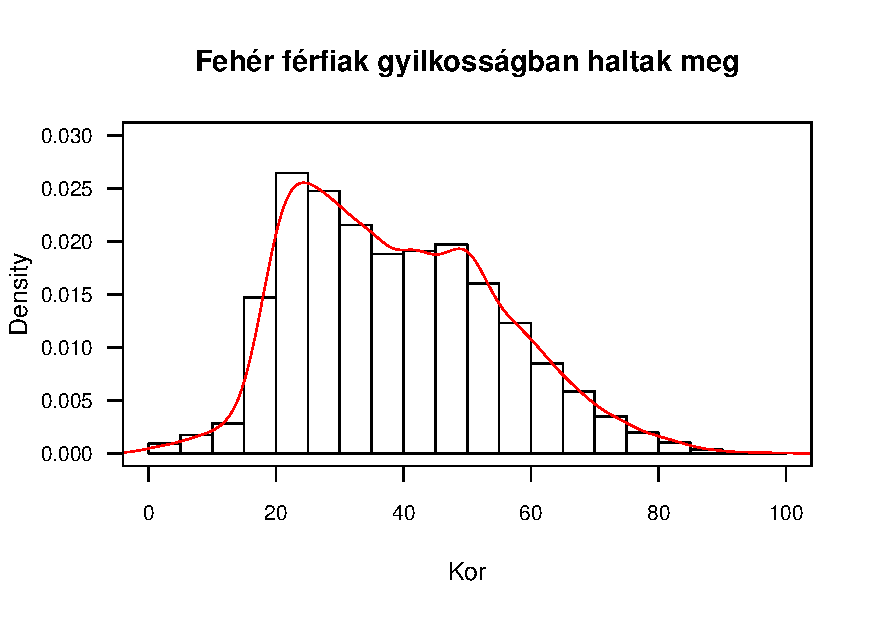
\includegraphics[width=65mm]{plot15.pdf}
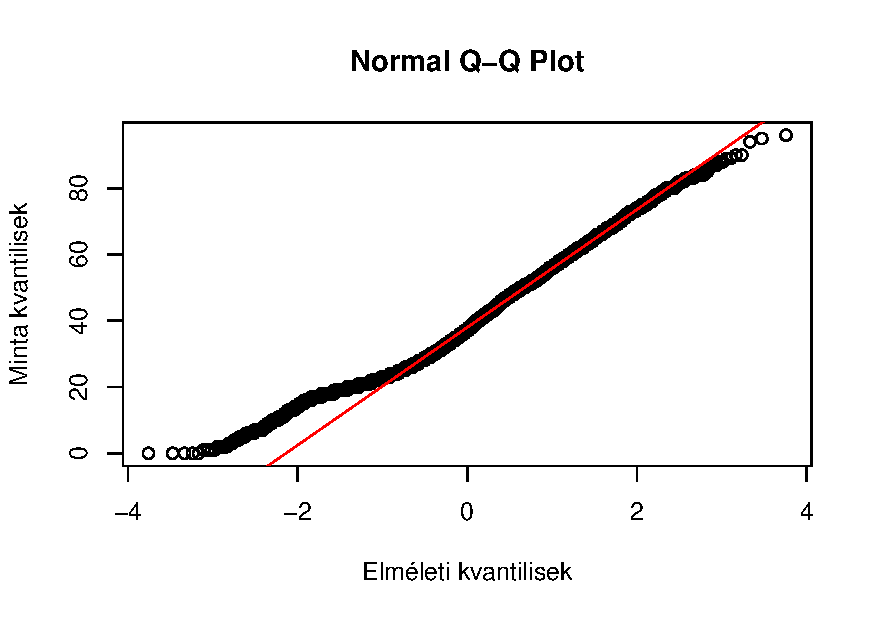
\includegraphics[width=65mm]{plot16.pdf}
\end{figure}

\subsubsection{Fehér nők gyilkosságban haltak meg}

Az eloszlás vastag szélű, alacsony szabadságfokkal.

\begin{figure}[!htb]
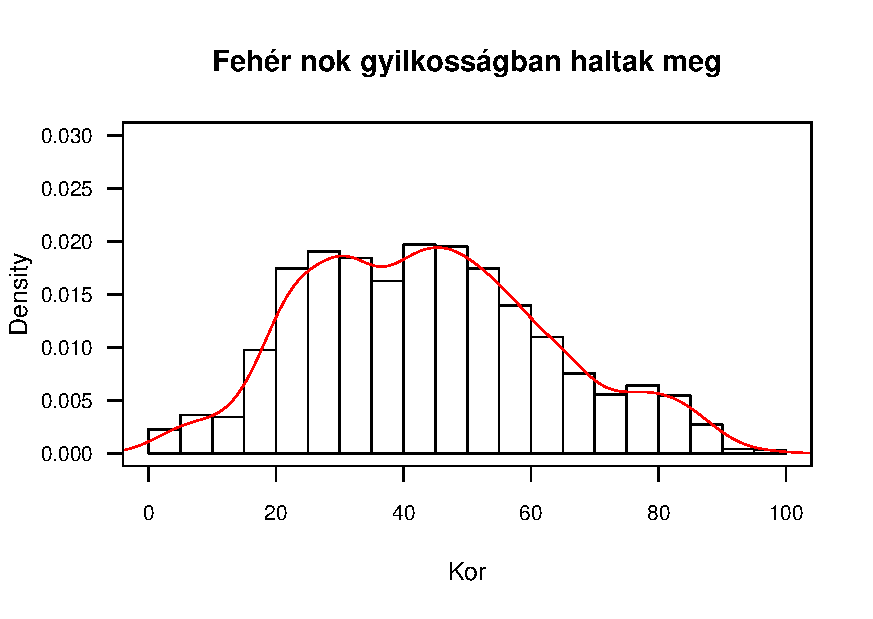
\includegraphics[width=65mm]{plot17.pdf}
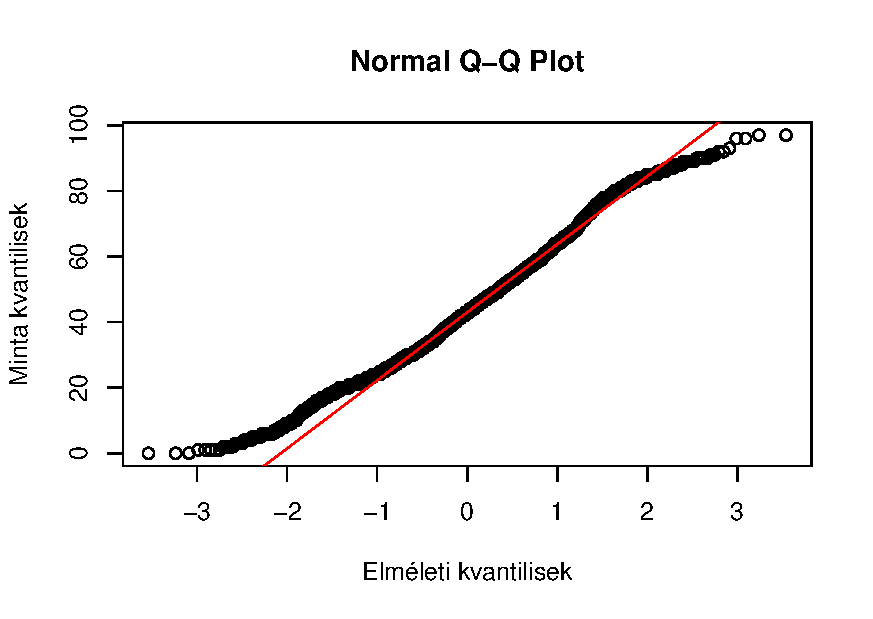
\includegraphics[width=65mm]{plot18.pdf}
\end{figure}

\subsubsection{Fekete férfiak gyilkosságban haltak meg}

Az eloszlás egyértelműen pozitív ferdeségű, valószínűleg ezek az adatok nagyban hozzájárulnak az általános eset tüskéjéhez.

\begin{figure}[!htb]
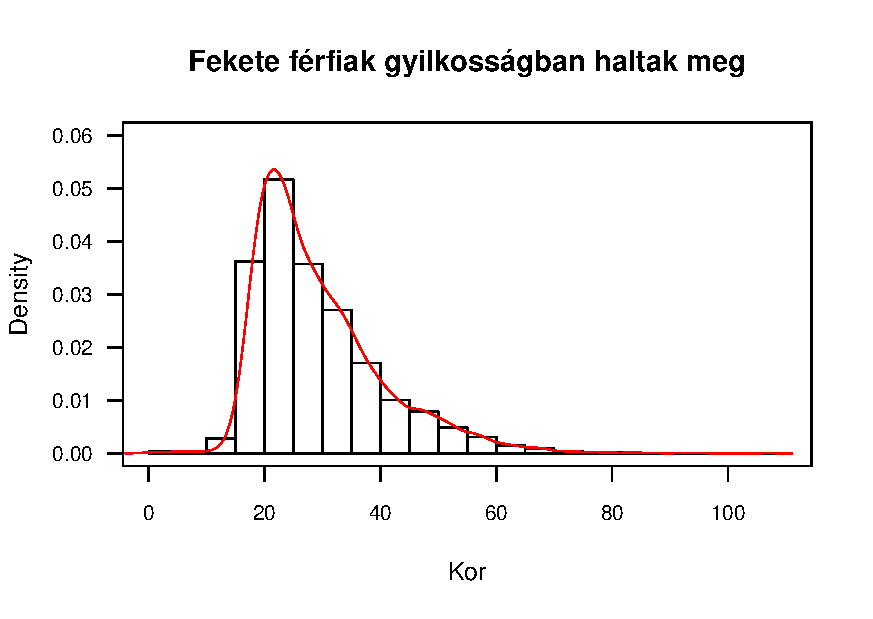
\includegraphics[width=65mm]{plot19.pdf}
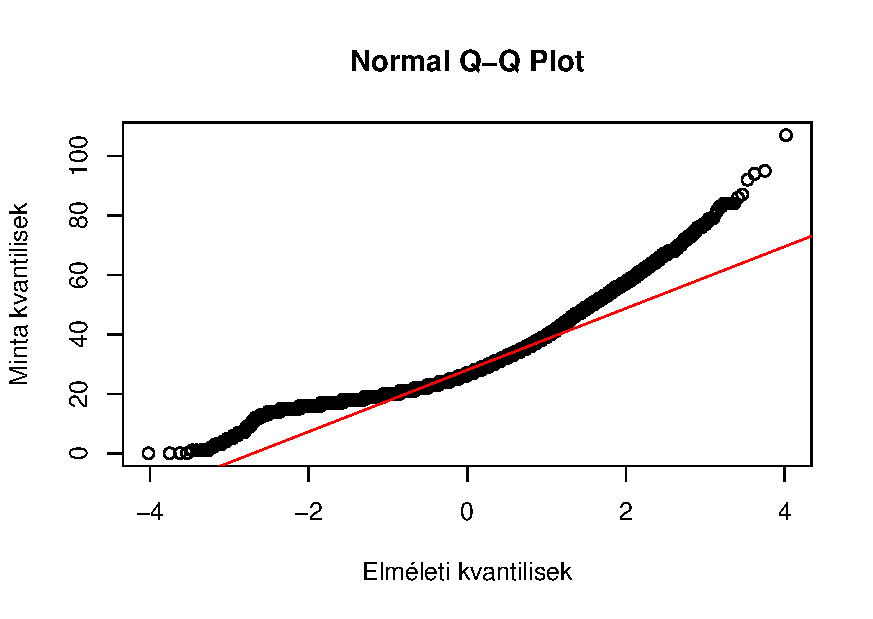
\includegraphics[width=65mm]{plot20.pdf}
\end{figure}

\subsubsection{Fekete nők gyilkosságban haltak meg}

Szintén pozitív ferdeségű eloszlás, ám a férfiak eseténél közelebb van a normális eloszláshoz.

\begin{figure}[!htb]
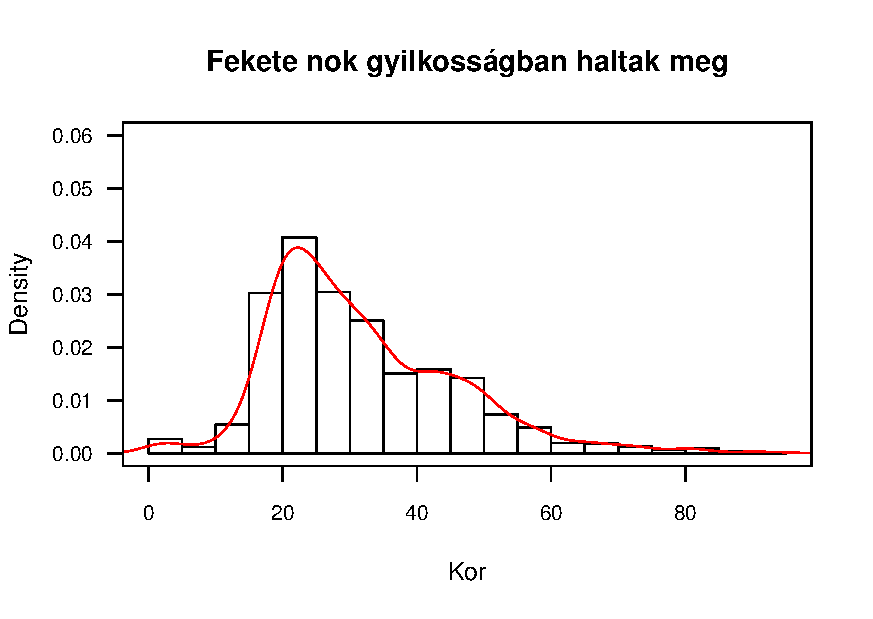
\includegraphics[width=65mm]{plot21.pdf}
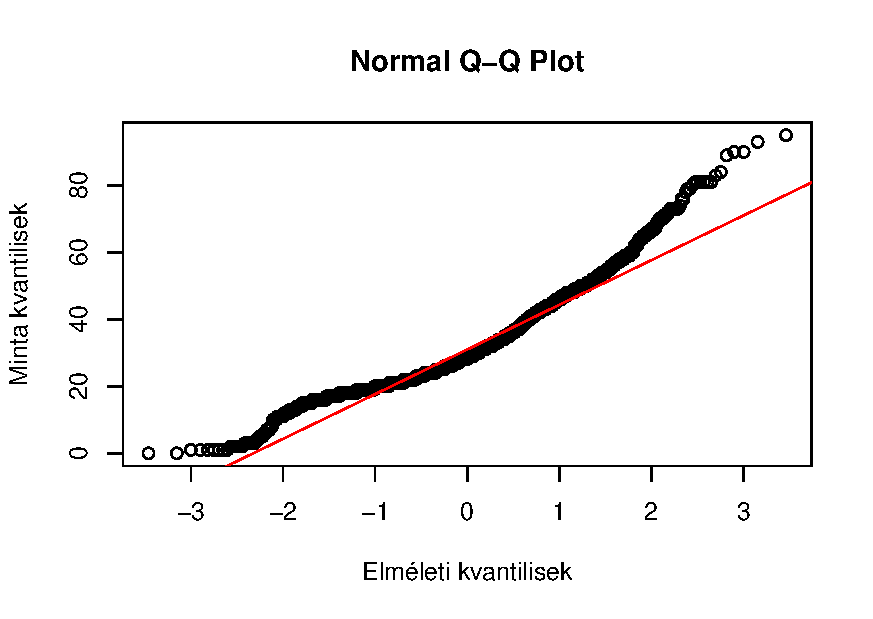
\includegraphics[width=65mm]{plot22.pdf}
\end{figure}

\subsubsection{Fehér férfiak öngyilkosságban haltak meg}

Vastagszélű eloszlás, nincs jelentős ferdesége.

\begin{figure}[!htb]
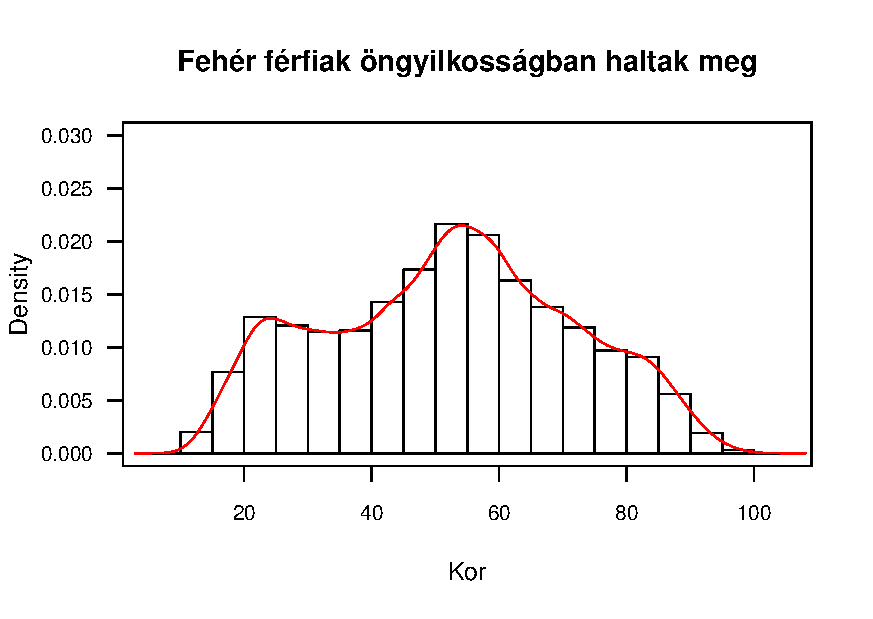
\includegraphics[width=65mm]{plot23.pdf}
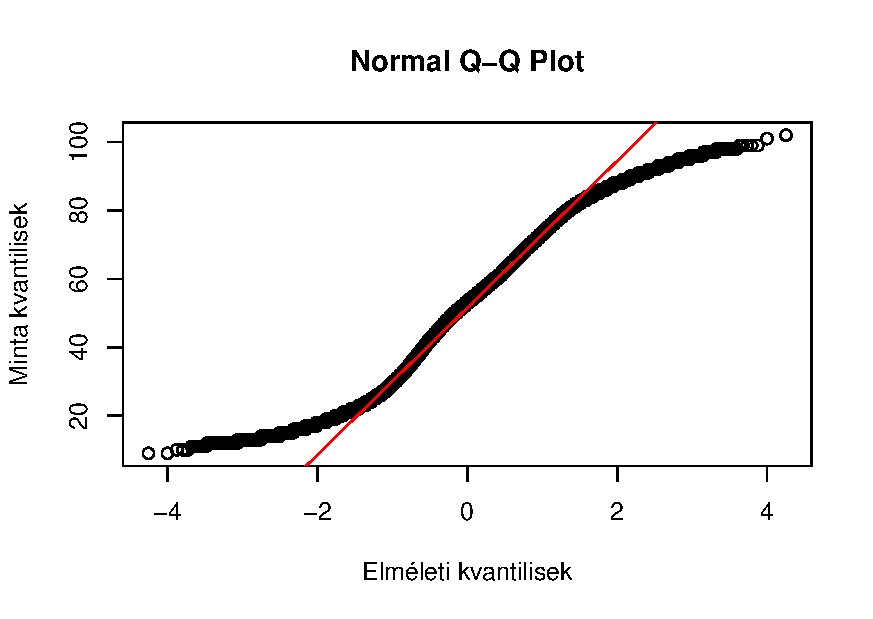
\includegraphics[width=65mm]{plot24.pdf}
\end{figure}

\subsubsection{Fehér nők öngyilkosságban haltak meg}

Az eloszlás vastag szélű, ugyanakkor eddig ez közelíti legjobban a normális eloszlást.

\begin{figure}[!htb]
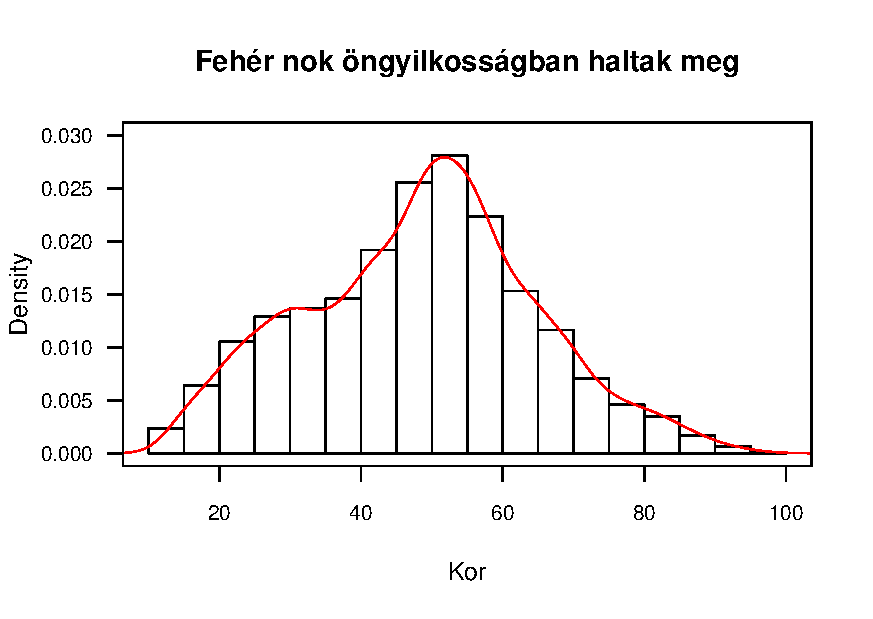
\includegraphics[width=65mm]{plot25.pdf}
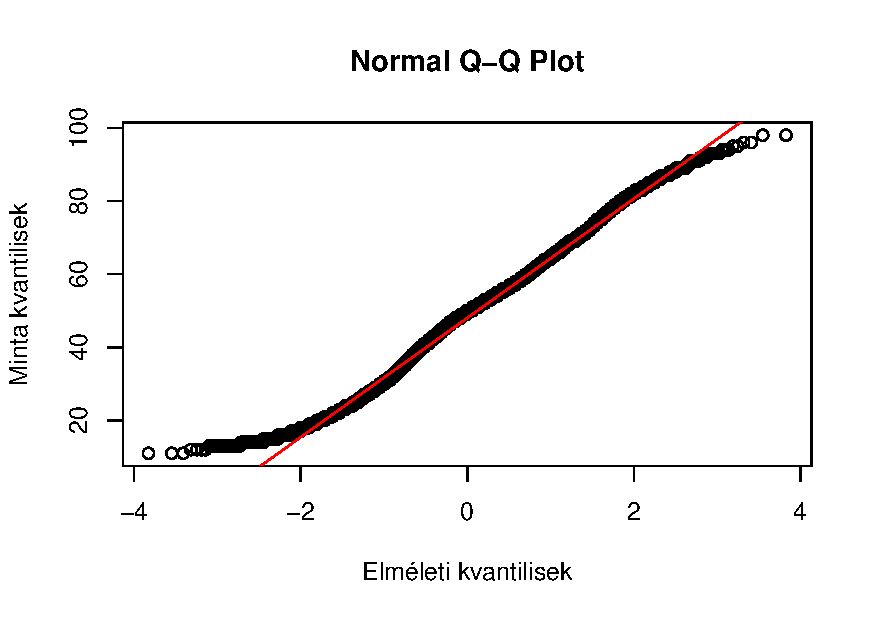
\includegraphics[width=65mm]{plot26.pdf}
\end{figure}

\subsubsection{Fekete férfiak öngyilkosságban haltak meg}

Az eloszlás nagyon hasonlít a fekete férfiak gyilkosságának adatai eloszlásához.

\begin{figure}[!htb]
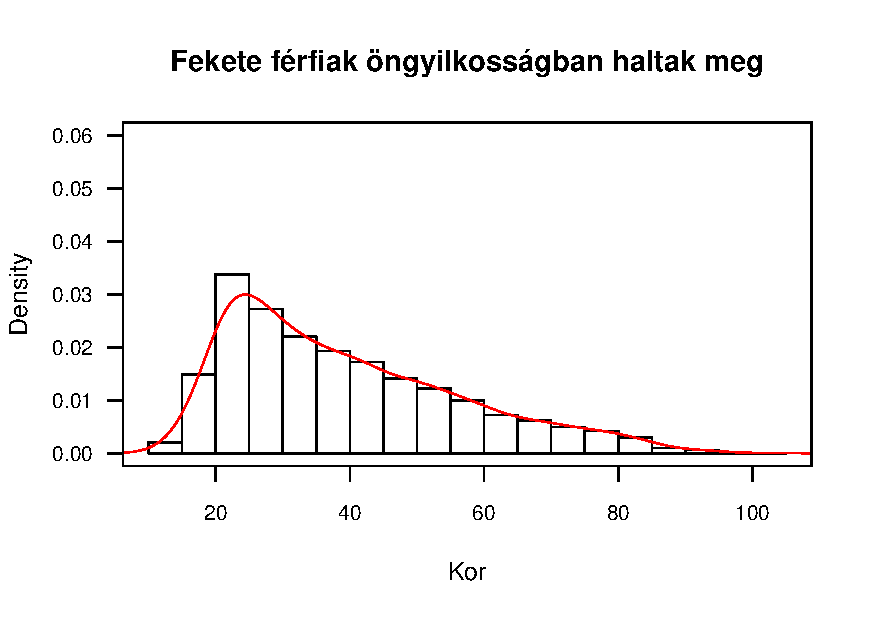
\includegraphics[width=65mm]{plot27.pdf}
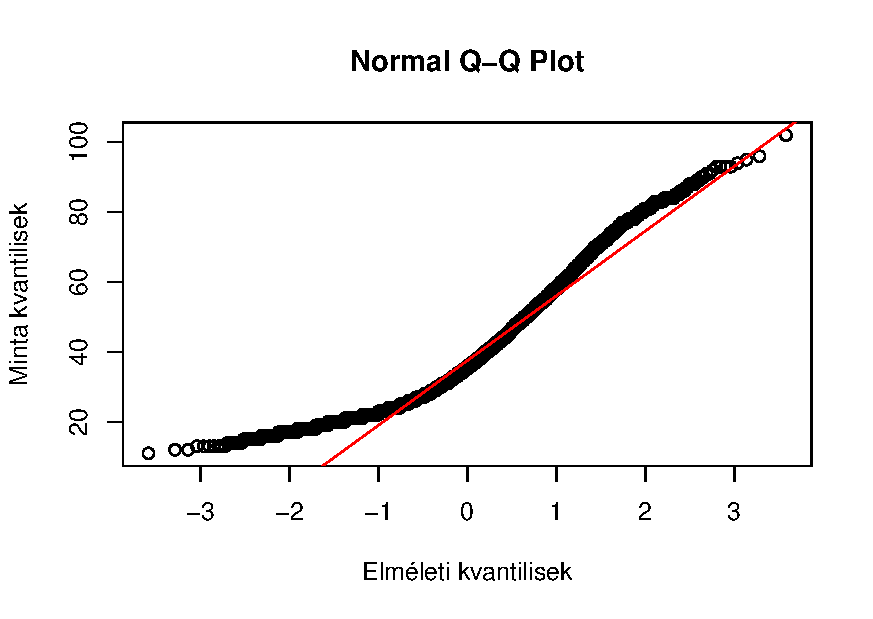
\includegraphics[width=65mm]{plot28.pdf}
\end{figure}

\newpage

\subsubsection{Fekete nők öngyilkosságban haltak meg}

Az eloszlás pozitív ferdeségő, ám igen jól közelíti a normális eloszlást.

\begin{figure}[!htb]
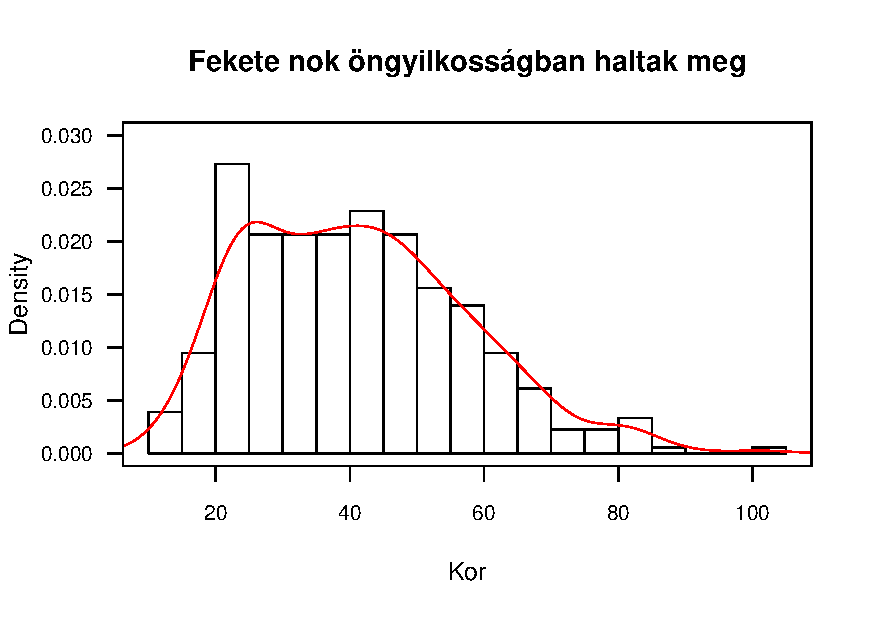
\includegraphics[width=65mm]{plot29.pdf}
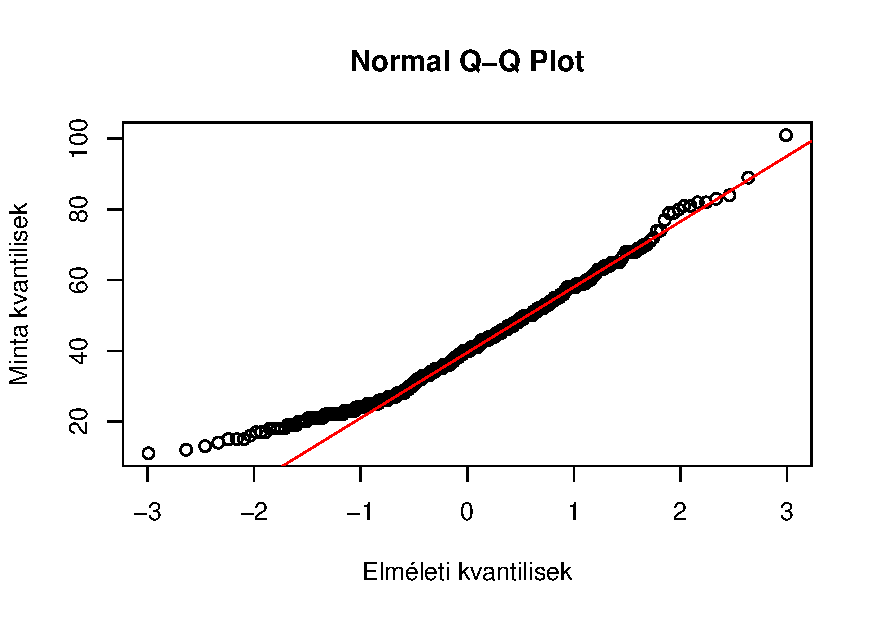
\includegraphics[width=65mm]{plot30.pdf}
\end{figure}

\section{Hipotézisvizsgálat}

\subsection{Egymintás t-próbák az előző adatokkal}

Az előző fejezetben normalitás szempontjából megvizsgált adatokra felírt egymintás t-próbák következnek. Jean Lemaire és Wharton School által $2000$ -ben írt, The Cost of Firearm Deaths in the United States: Reduced Life Expectancies and Increased Insurance Costs című tanulmányában megjelenő átlagéletkorok alapján vizsgálom a $2012$ - $2014$ közti adatokat. \par
A nullhipotézis az lesz minden esetben, hogy a fegyver által meghalt emberek átlagéletkora csökkent a $2000$-es adatokhoz képest. \par
Legyen  $\alpha = 0.05$.

\subsubsection{Fehér férfiak gyilkosságban haltak meg}
Ebben az esetben elvethetjük a nullhipotézisünket, ugyanis  $t = 32.156$ továbbá  $p < 2.2e-16$, ami alapján $p < \alpha$.

\subsubsection{Fehér nők gyilkosságban haltak meg}
Ebben az esetben elvethetjük a nullhipotézisünket, ugyanis  $t = 12.144$ továbbá  $p < 2.2e-16$, ami alapján $p < \alpha$.

\subsubsection{Fekete férfiak gyilkosságban haltak meg}
Ebben az esetben nem tudjuk elvetni a nullhipotézisünket, ugyanis  $t = -106.32$ továbbá  $p = 1$, ami alapján $p > \alpha$.

\subsubsection{Fekete nők gyilkosságban haltak meg}
Ebben az esetben nem tudjuk elvetni a nullhipotézisünket, ugyanis  $t = -0.36915$ továbbá  $p = 0.644$, ami alapján $p > \alpha$.

\subsubsection{Fehér férfiak öngyilkosságban haltak meg}
Ebben az esetben elvethetjük a nullhipotézisünket, ugyanis  $t = 35.834$ továbbá  $p < 2.2e-16$, ami alapján $p < \alpha$.

\subsubsection{Fehér nők öngyilkosságban haltak meg}
Ebben az esetben elvethetjük a nullhipotézisünket, ugyanis  $t = 14.047$ továbbá  $p < 2.2e-16$, ami alapján $p < \alpha$.

\subsubsection{Fekete férfiak öngyilkosságban haltak meg}
Ebben az esetben elvethetjük a nullhipotézisünket, ugyanis  $t = 8.1931$ továbbá  $p < 2.2e-16$, ami alapján $p < \alpha$.

\subsubsection{Fekete nők öngyilkosságban haltak meg}
Ebben az esetben elvethetjük a nullhipotézisünket, ugyanis  $t = 3.2883$ továbbá  $p = 0.0005539$, ami alapján $p < \alpha$.

\subsection{Kétmintás t-próba}

A tesztet fegyver által meghalt férfiak és nők átlagéletkora között végzem. A teszt elvégezhető, ugyanis a két adathalmaz független egymástól. A nullhipotézis az lesz, hogy a fegyver által meghalt nők átlagéletkora magasabb, mint a fegyver által meghalt férfiak átlagéletkora. Legyen $\alpha = 0.05$ ismét. \par
A teszt eredménye: $t = -1.0674$, $p = 0.8571$ vagyis mivel $p > \alpha$, így a nullhipotézisünket nem tudjuk elutasítani, tehát feltételezhetjük, hogy a férfiak átlagéletkora alacsonyabb mint a nőké, a megadott feltételek mellett.

\subsection{Khí-négyzet próbák}

A khí-négyzet próba azt ellenőrzi, hogy a két kategória típusú változó független-e egymástól. Ismét legyen $\alpha = 0.05$.

\begin{minipage}{0.45\textwidth}
A Khí-próbát a nem és szándék változókra kiszámolva azt kapjuk, hogy $X-squared = 66.416$ és $p = 3.784e-15$, tehát van összefüggés a két változó között, ugyanis $p < \alpha$.
\end{minipage}
\begin{minipage}{0.5\textwidth}
\begin{figure}[H]
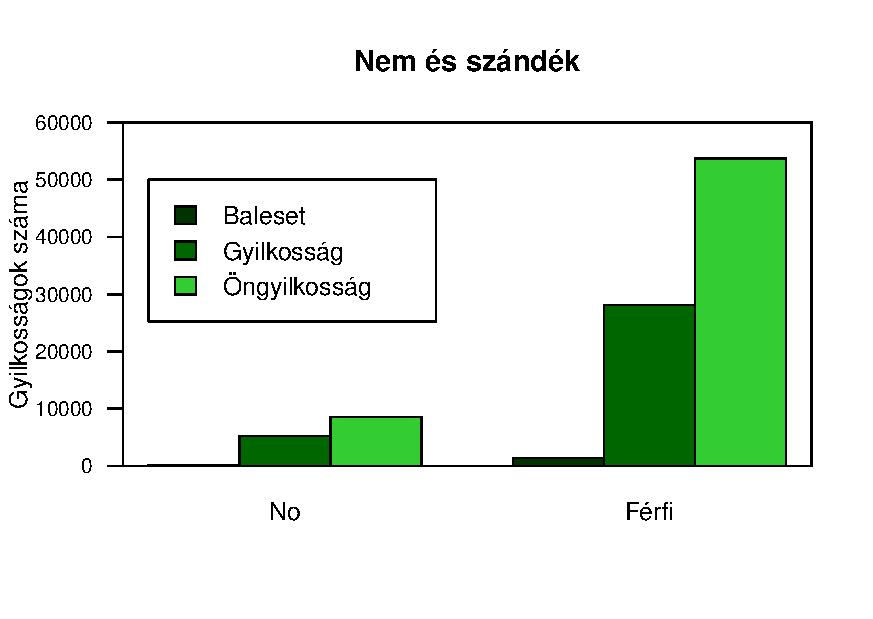
\includegraphics[width=65mm]{plot31.pdf}
\end{figure}
\end{minipage} \hfill


\begin{minipage}{0.5\textwidth}
\begin{figure}[H]
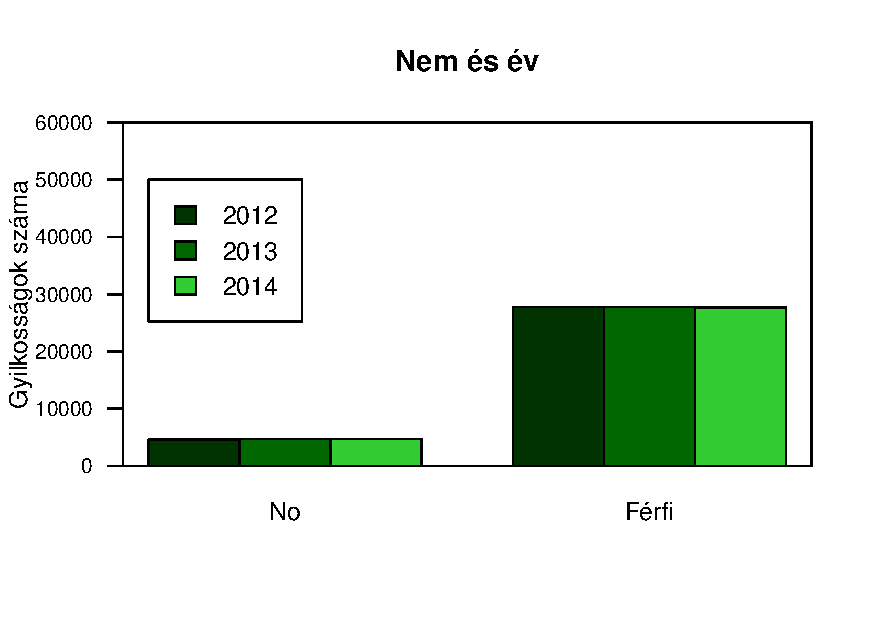
\includegraphics[width=65mm]{plot32.pdf}
\end{figure}
\end{minipage} \hfill
\begin{minipage}{0.45\textwidth}
A Khí-próbát a nem és év változókra kiszámolva azt kapjuk, hogy $X-squared = 2.3868$ és $p = 0.3032$, tehát nincs összefüggés a két változó között, ugyanis $p > \alpha$.
\end{minipage}

\newpage
\tableofcontents

\end{document}

